\chapter{Analyse et spécification des besoins}

\section{Introduction}
Nous réservons le deuxième chapitre pour détailler le cadre du projet, par une étude et critique de l’existant puis présenter la solution envisagée par le cahier de charges proposé.
Ensuite,nous allons identifier les acteurs qui interagissent directement avec l’ensemble de notre application, puis nous présentons dans ce qui suit les besoins fonctionnels classés par acteur ainsi que les besoins non fonctionnels et le diagramme de classes et séquence du projet.
% Une section
\section{\'Etude et critique de l'existant}
Il existe de nos jour un grand nombre de logiciels de génération de formulaires en ligne, ces  logiciels d’enquête  qui ne nécessitent aucune connaissance en programmation, peuvent s’avérer très utiles dans l’élaboration d’un questionnaire en ligne.\\
Ces derniers peuvent être des bons outils pour répondre mieux à nos attentes mais peuvent par conséquent présenter certaines limites dans leur utilisation.\\
Nous proposons une liste non exhaustive de quelques outils de génération de formulaires en ligne qui sont les leaders dans le marché accompagnée d'une brève analyse des avantages et des limites :\\
- \textbf{Google Forms}: Les formulaires Google sont des outils très pratiques par leur simplicité de mise en place et leur exploitation, aucune limite au nombre de questionnaires et au nombre de répondants, ils sont idéals pour les débutants, par conséquent la mise en page des questionnaires n’est que très peu personnalisable et ses serveurs sont localisés à l’étranger, les données seront soumises aux lois de ce même pays qu'il faut vérifier que cela soit compatible avec les exigences des comités d'éthiques.\\%te7ki b s3ib xD
- \textbf{LimeSurvey}: Un générateur de formulaire permet de créer rapidement et de manière intuitive de puissants questionnaires et enquêtes en ligne. Le questionnaire est hébergé sur le serveur de l’utilisateur mais ça reste toujours un outils considéré comme non personnalisé et que nous pouvons pas l'intégrer facilement dans des applications privées. 

\section{Solution proposée}
Tenant compte de l’étude approfondie de l’existant nous allons élaborer la solution proposée par SOFIA Technologies à mettre en oeuvre qui réponds à ces deux exigences : \\
- Développer un générateur de formulaire personnalisé qui garanti les besoins définis dans le cahier des charges.\\
- Proposer la solution sous forme d'un POC qui a pour but d’analyser sur une période définie et en situation réelle la mise en place d’une solution d’affichage dynamique dans le but de valider la conformité du projet avec les objectifs fixés, et plus globalement, avec le cahier des charges élaboré {Proof Of Concept \cite{webArticle2}}
\section{Identification des acteurs du système}
Les acteurs sont les entités externes qui interagissent avec le système. Notre projet comporte principalement deux acteurs :\\
- \textbf{Administrateur}: C’est l’acteur principal, il est responsable de la gestion des utilisateurs, des formulaires et des réponses de l’application.\\
- \textbf{Utilisateur}: Il s’agit d’un acteur principal aussi, il assure la consultation et la soumission des formulaires disponibles.
        
\section{Identification des besoins}
    % Une sous section
    \subsection{Besoins fonctionnels}
Les besoins fonctionnels représentent les services qui doivent être offerts et qui seront implémentés par l’application. Ainsi, cette application doit couvrir principalement les
besoins fonctionnels suivants :
\begin{itemize}
    \item S’authentifier : L’utilisateur peut créer un compte personnel et se connecter grâce à son login et mot de passe.
\end{itemize}
Pour l’administrateur :
\begin{itemize}
    \item Gérer les formulaires et leurs questions: cette étape consiste à faire les opérations CRUD pour un formulaire donné.
    \item Consulter la liste des formulaires : il peut visualiser tous les formulaires qu'il a crées.
    \item Consulter l’ensemble des réponses : L’administrateur peut consulter les réponses des utilisateurs aux différents formulaires qu'il a crées,les supprimer et même télécharger la liste des réponses.
\end{itemize}

Pour l'utilisateur:
\begin{itemize}
\item Consulter la liste des formulaires : L’utilisateur peut visualiser tous les formulaires crées par l’administrateur.
\item Soumettre un formulaire: il peut répondre aux questions d'un formulaire, modifier ses réponses et les soumettre.
\end{itemize}
    % Une deuxième sous section1
    \subsection{Besoins non fonctionnels}
      Dans le cadre de ce travail, notre application devra être :
\begin{itemize}
 \item  \textbf{Performante} : l’administrateur ne peut gérer les formulaires et les utilisateurs qu’après authentification et même cas pour les utilisateurs pour répondre aux formulaires.
 \item \textbf{Ergonomique } : Il s’agit d’une application présentant des interfaces utilisateur conviviales bien structurée et simple à manipuler
 \item  \textbf{Rapide et fluide} : Ce besoin envisage avec une vitesse de navigation minime, temps de réponse rapide et temps d’affichage optimisé.
\end{itemize}
\section{Conception}
\subsection{Le diagramme de classe et diagramme de cas d’utilisation}
Dans cette section nous présentons le diagramme de cas d’utilisation des fonctionnalités déjà mentionnées ainsi que le diagramme de classes.\\
Le diagramme de cas d’utilisation général de la figure  (\ref{casgeneral}) permet d’avoir une vue globale du fonctionnement de notre système à réaliser.
\begin{figure}[H]
    \centering
    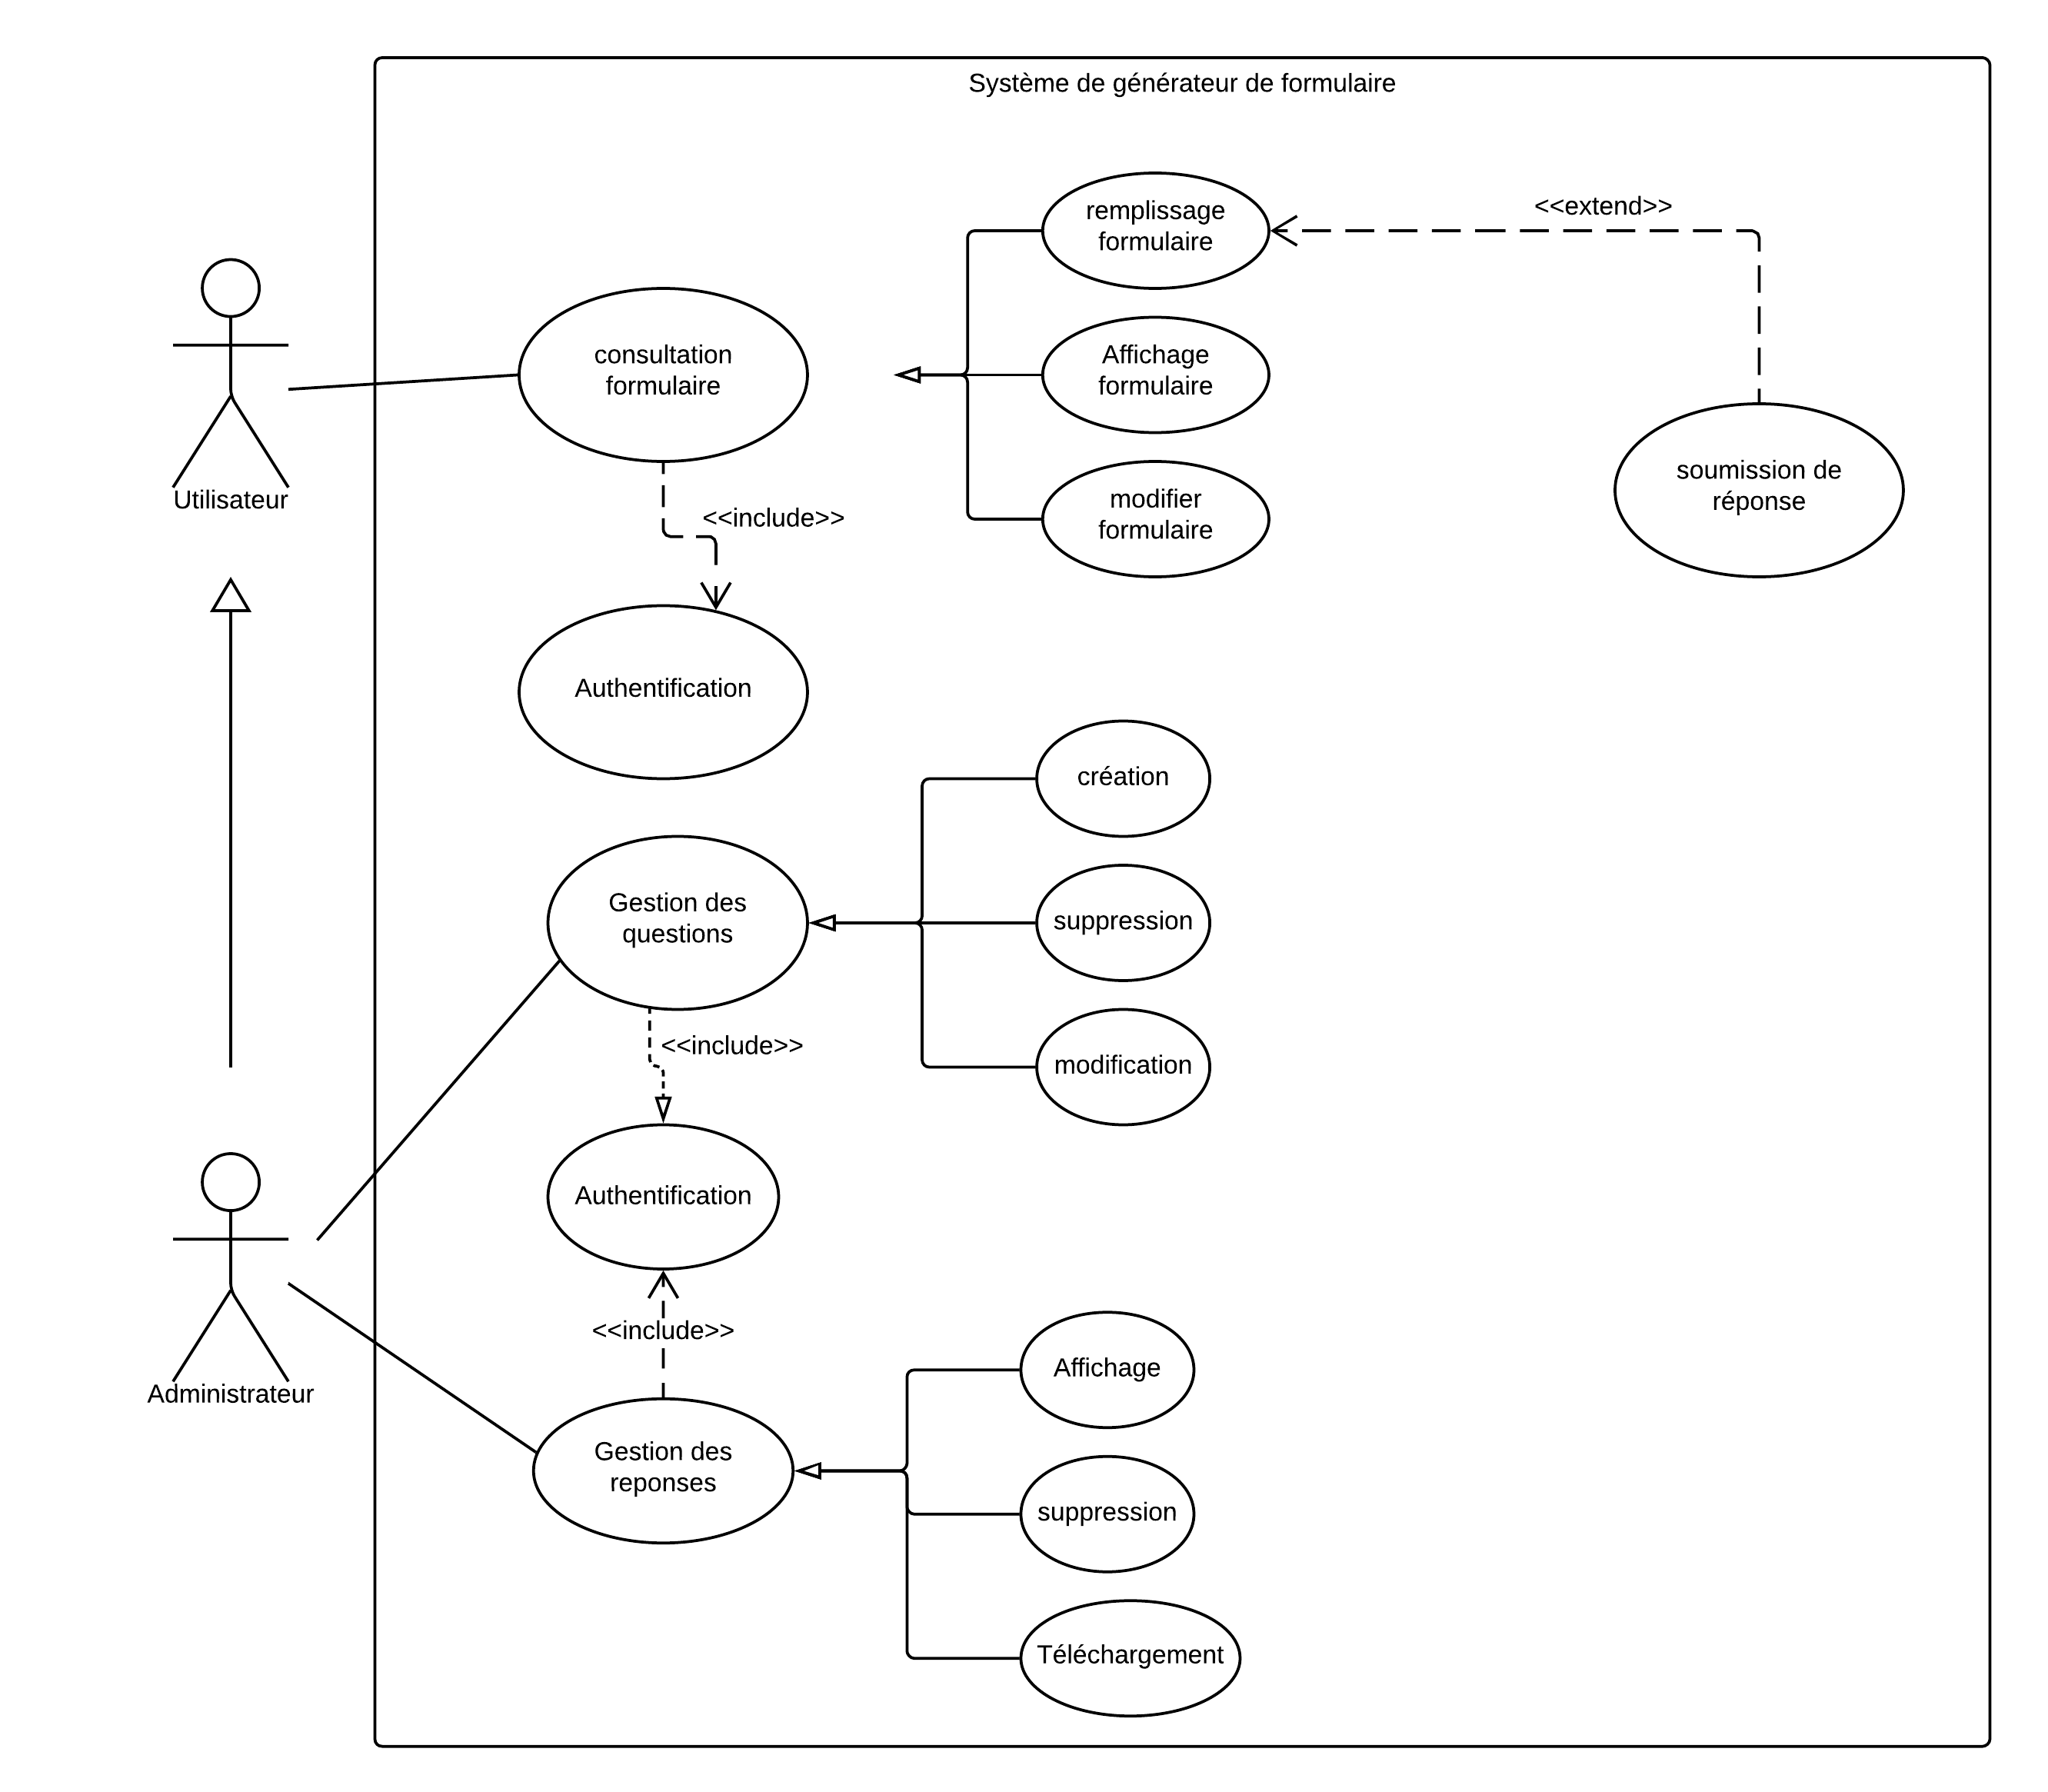
\includegraphics[width=14cm, height=8cm]{img/Diag_usecase.png}
    \caption{Digramme de cas d'utilisation général}
    \label{casgeneral}
\end{figure}

La figure (\ref{ClasseGeneral}) présente le diagramme de classes de notre projet.
\begin{figure}[H]
    \centering
    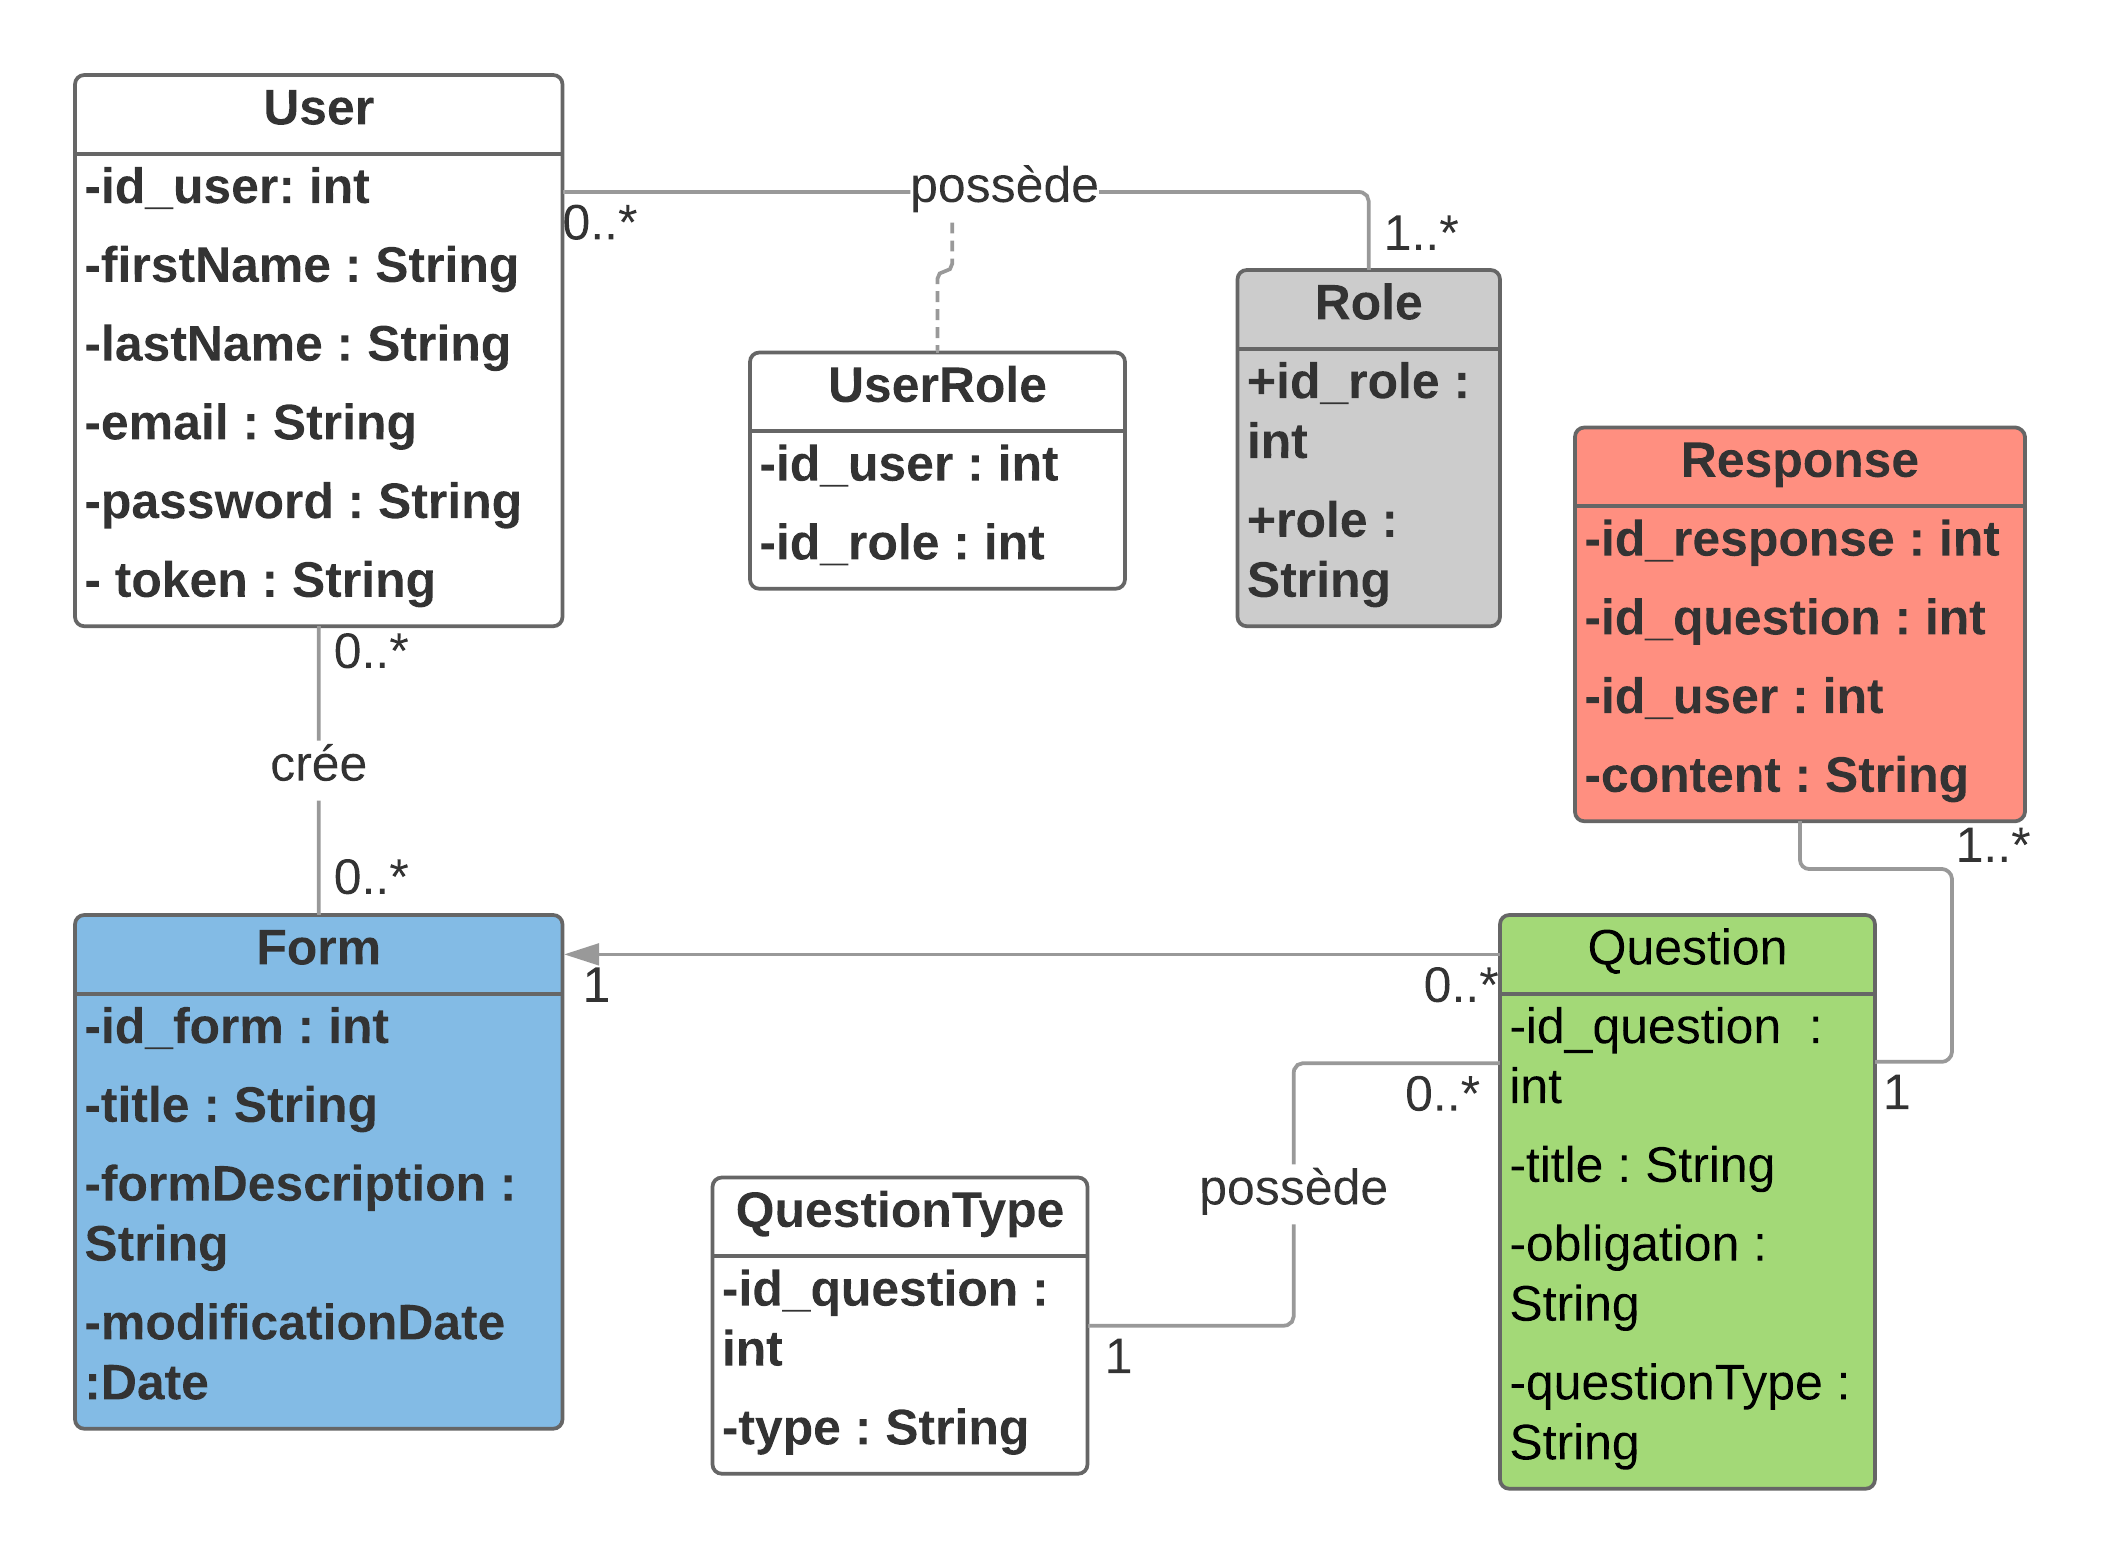
\includegraphics[width=14cm, height=8cm]{img/DiagClasse.png}
    \caption{Digramme de classes général}
   \label{ClasseGeneral}
\end{figure}

\subsection{Identification des scénarios}
  
Le tableau \ref{tabGererOffre} présente la description détaillée du cas d'utilisation "s'inscrire".
    \begin{longtable}{|p{4cm}|p{10.25cm}|}
	\hline
	\textbf{Nom} & Authentification\\ \hline
	\textbf{Acteur}& L'utilisateur. \\ \hline
	\textbf{Description} & Permettre aux utilisateurs de créer des comptes. \\ \hline
	\textbf{Pré-condition} & 1. L'utilisateur devrait consulter la page d'inscription.L'utilisateur ne doit pas être déjà enregistré.\\
	\hline \textbf{Scénario nominal} & 1. L'utilisateur saisit son username.\\
	& 2. L'utilisateur saisit son mot de passe.
	\\ \hline
	\textbf{Scénario d'exception} &  Si l'utilisateur saisit un email ou un username erroné, il sera invité à saisir son login de nouveau.\\ \hline
	\textbf{Post-condition} & L'utilisateur devient authentifié par l'intermédiaire d'un token.\\\hline
	\caption{ Description du processus d'inscription}\label{tabGererOffre}
	\end{longtable}
\section{Schéma de la base de données}
Pour pouvoir commencer la partie développement, il faut bien comprendre la structure de notre base de données c’est-à-dire les entités et les associations.\\
A l'aide du système de gestion de bases de données relationnelles MySQL, nous avons pu installer notre serveur de base de données. La figure \ref{schémaDB} illustre le schéma de la base de données en détaillant les attributs de chaque table.
 \begin{figure} [H]
    \centering
         \begin{center}
             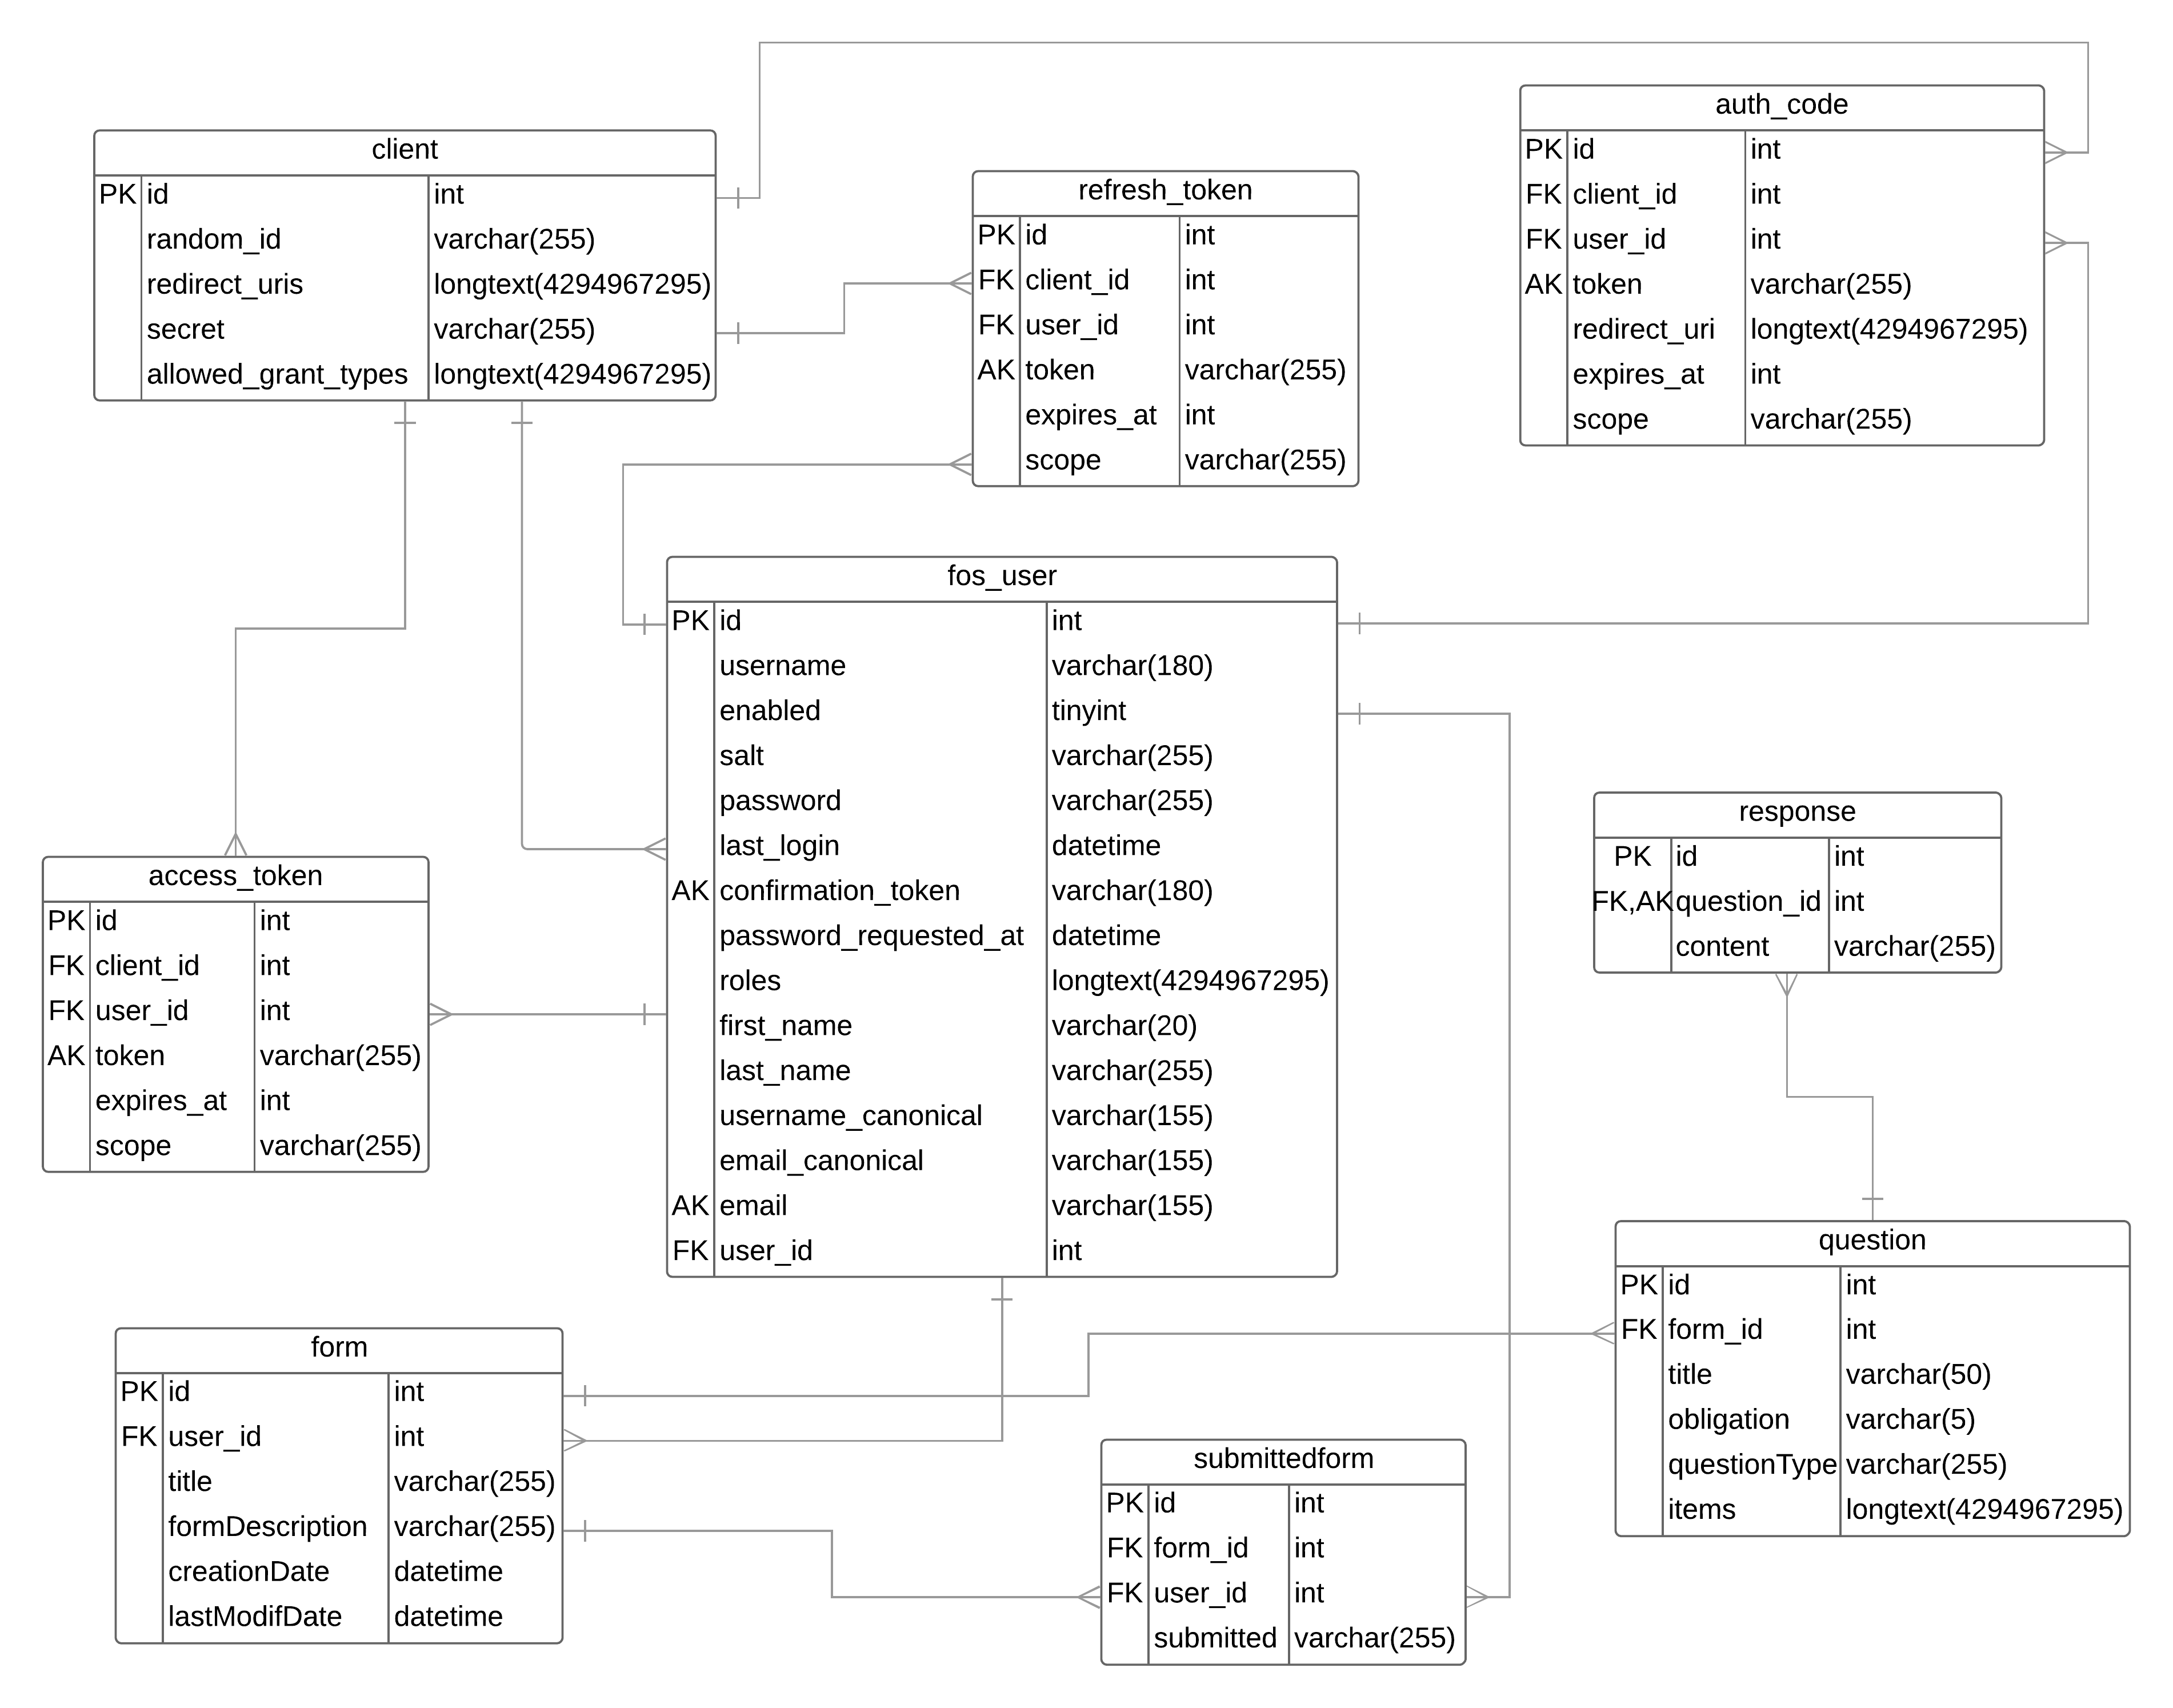
\includegraphics [width=16cm,height=9cm] {SprintImage/DB_schema}
            \caption{Schéma de la base de données}
            \label{schémaDB}
        \end{center}
    \end{figure}
\subsection{Diagrammes de séquence}
Dans cette partie, nous allons modéliser les fonctionnalités du premier sprint sous forme d’une séquence de messages échangés entre l’acteur et le système.\\
\textbf{Diagramme de séquence système « S’authentifier »}\\
La figure \ref{séqAuth} représente l’enchaînement du cas d’utilisation « S’authentifier ». Le user ou l'administrateur demande son authentification en saisissant ses identifiants
(username, password). Le système vérifie si les identifiants sont corrects ou non. Une fois les coordonnées sont valides,un token(jeton d'authentification) est envoyé du back-end et le User sera amené à la page d’accueil. Dans le cas contraire, un message d’erreur sera affiché en lui indiquant le problème.
\begin{figure} [H]
    \centering
         \begin{center}
             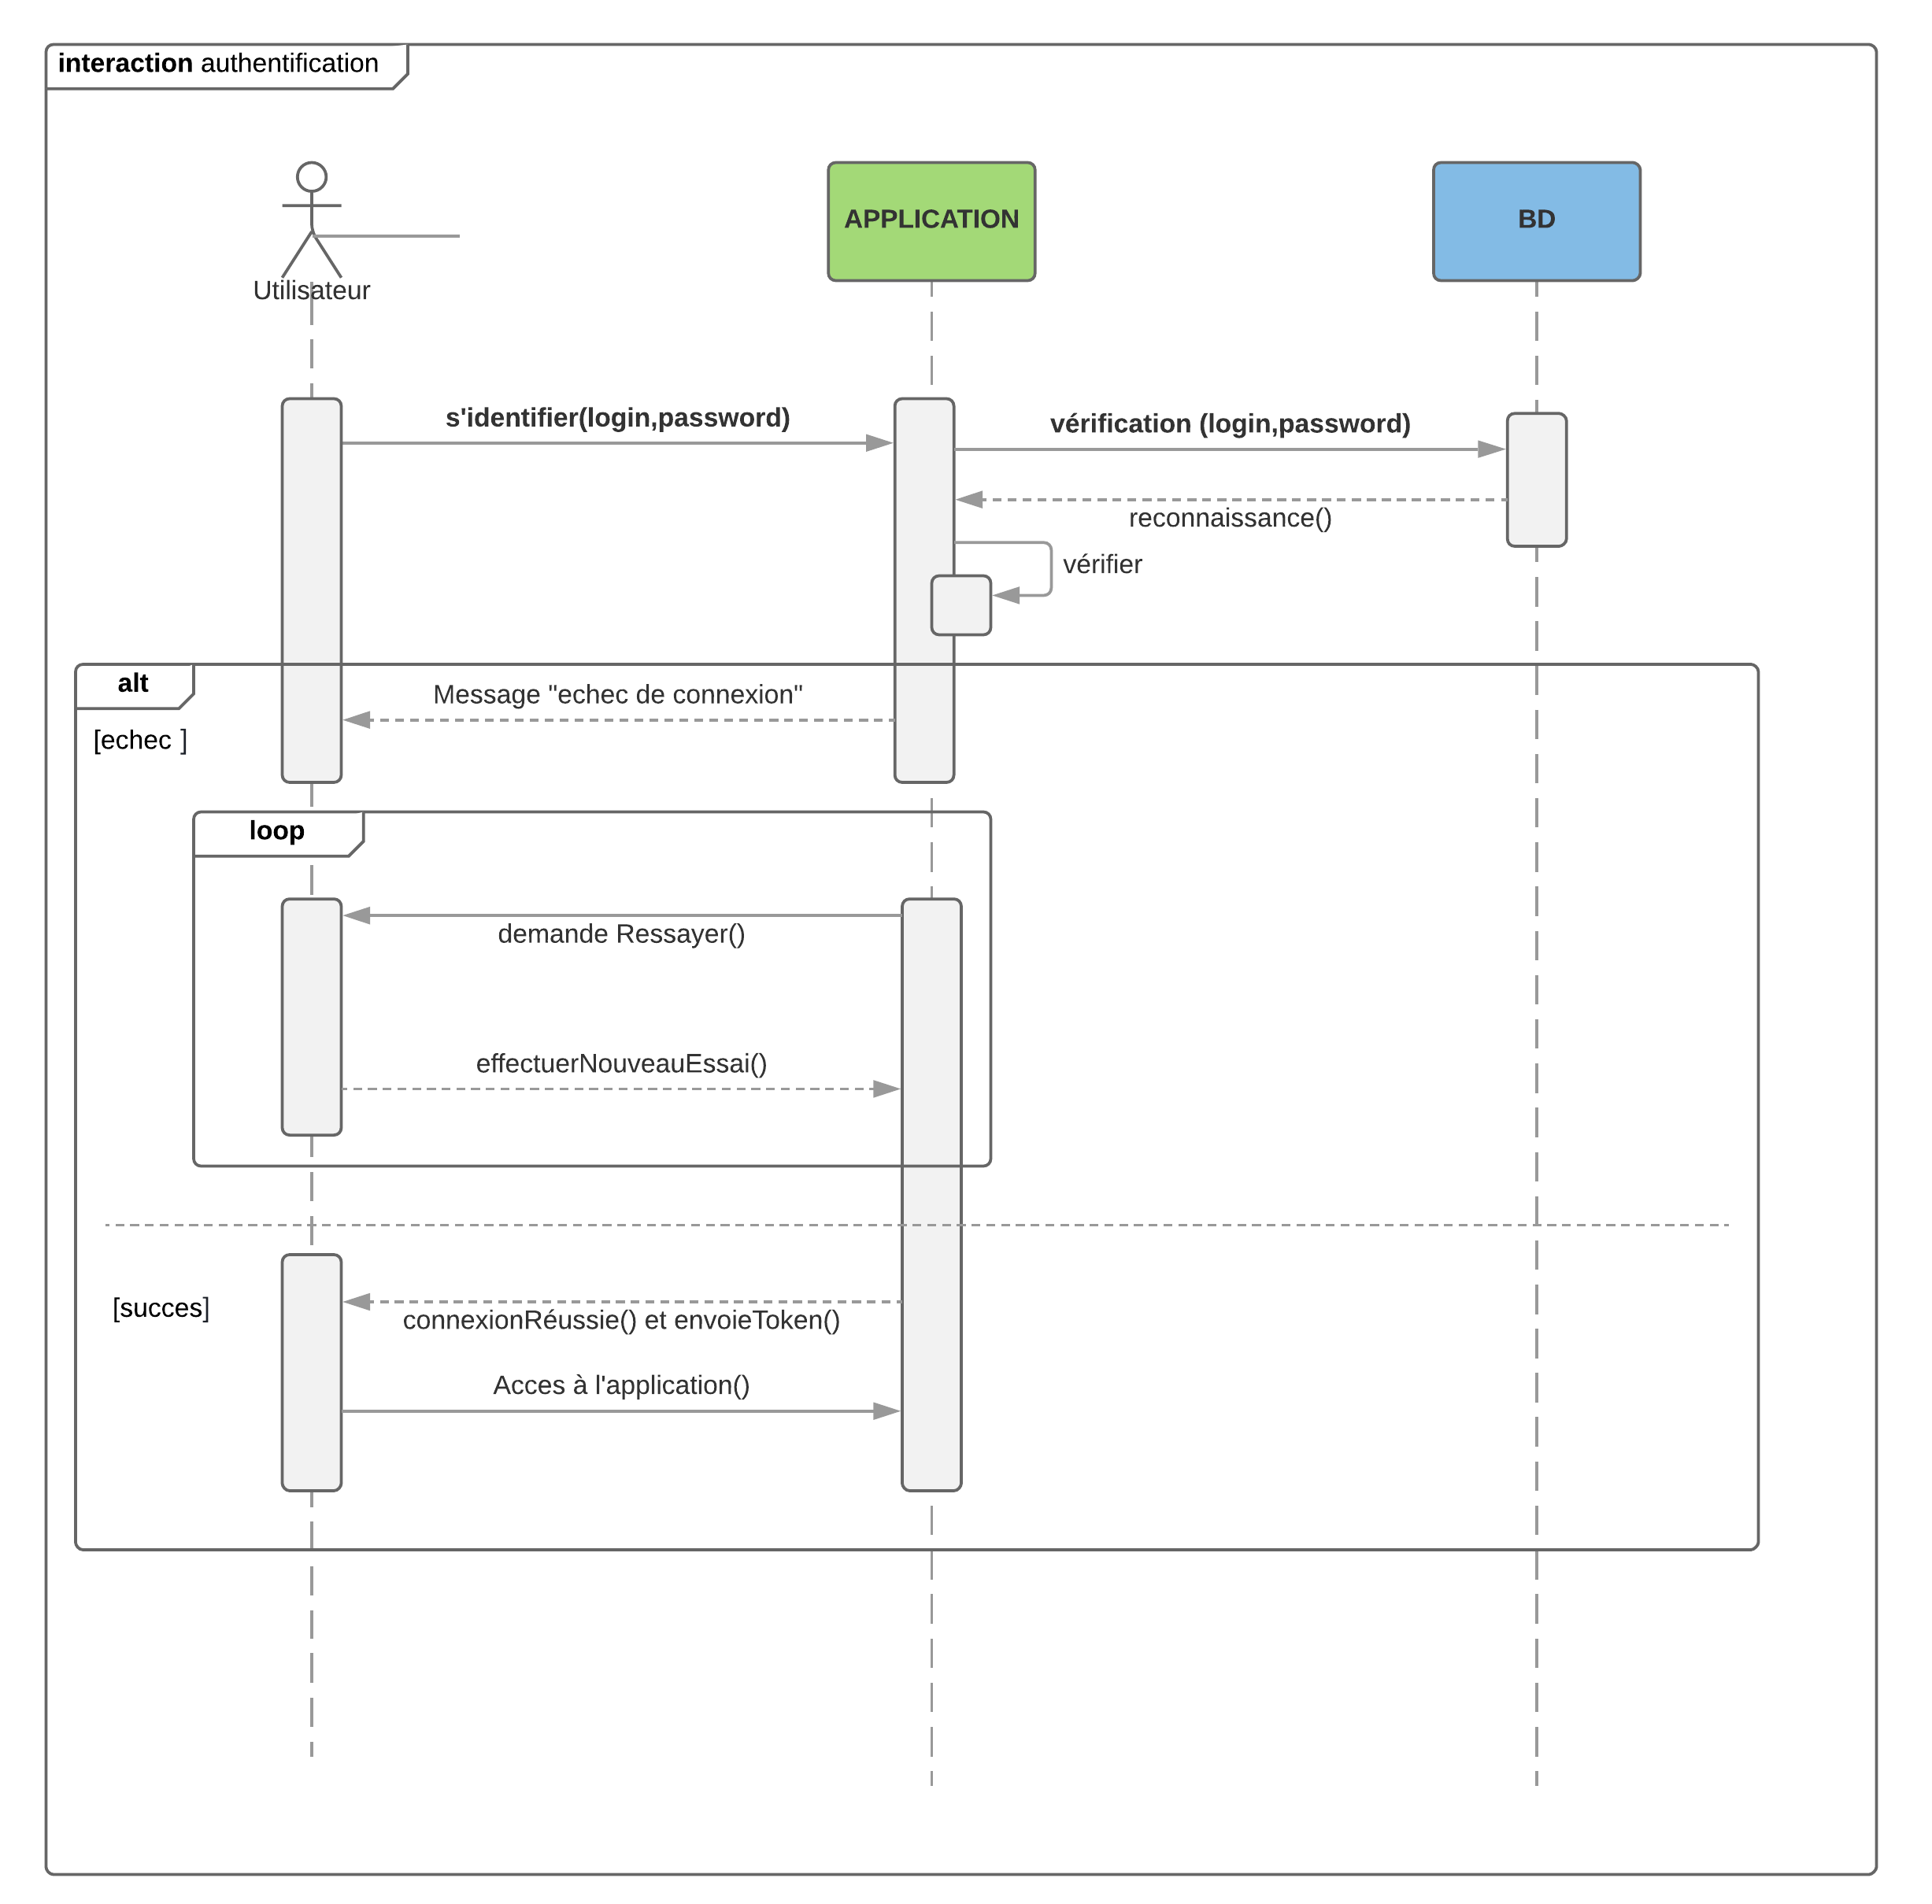
\includegraphics [width=15cm,height=11cm] {SprintImage/Diagramme_seq_Auth}
            \caption{Diagramme de séquence système « S’authentifier »}
            \label{séqAuth}
        \end{center}
    \end{figure}
    \newpage
\subsection{Diagramme de séquence système « Soumettre la réponse d'un formulaire »}
Le diagramme de la figure \ref{fig4}, représente les étapes qu'un utilisateur doit suivre afin de soumettre sa réponse à un questionnaire choisit.  
  \begin{figure} [H]
    \centering
         \begin{center}
             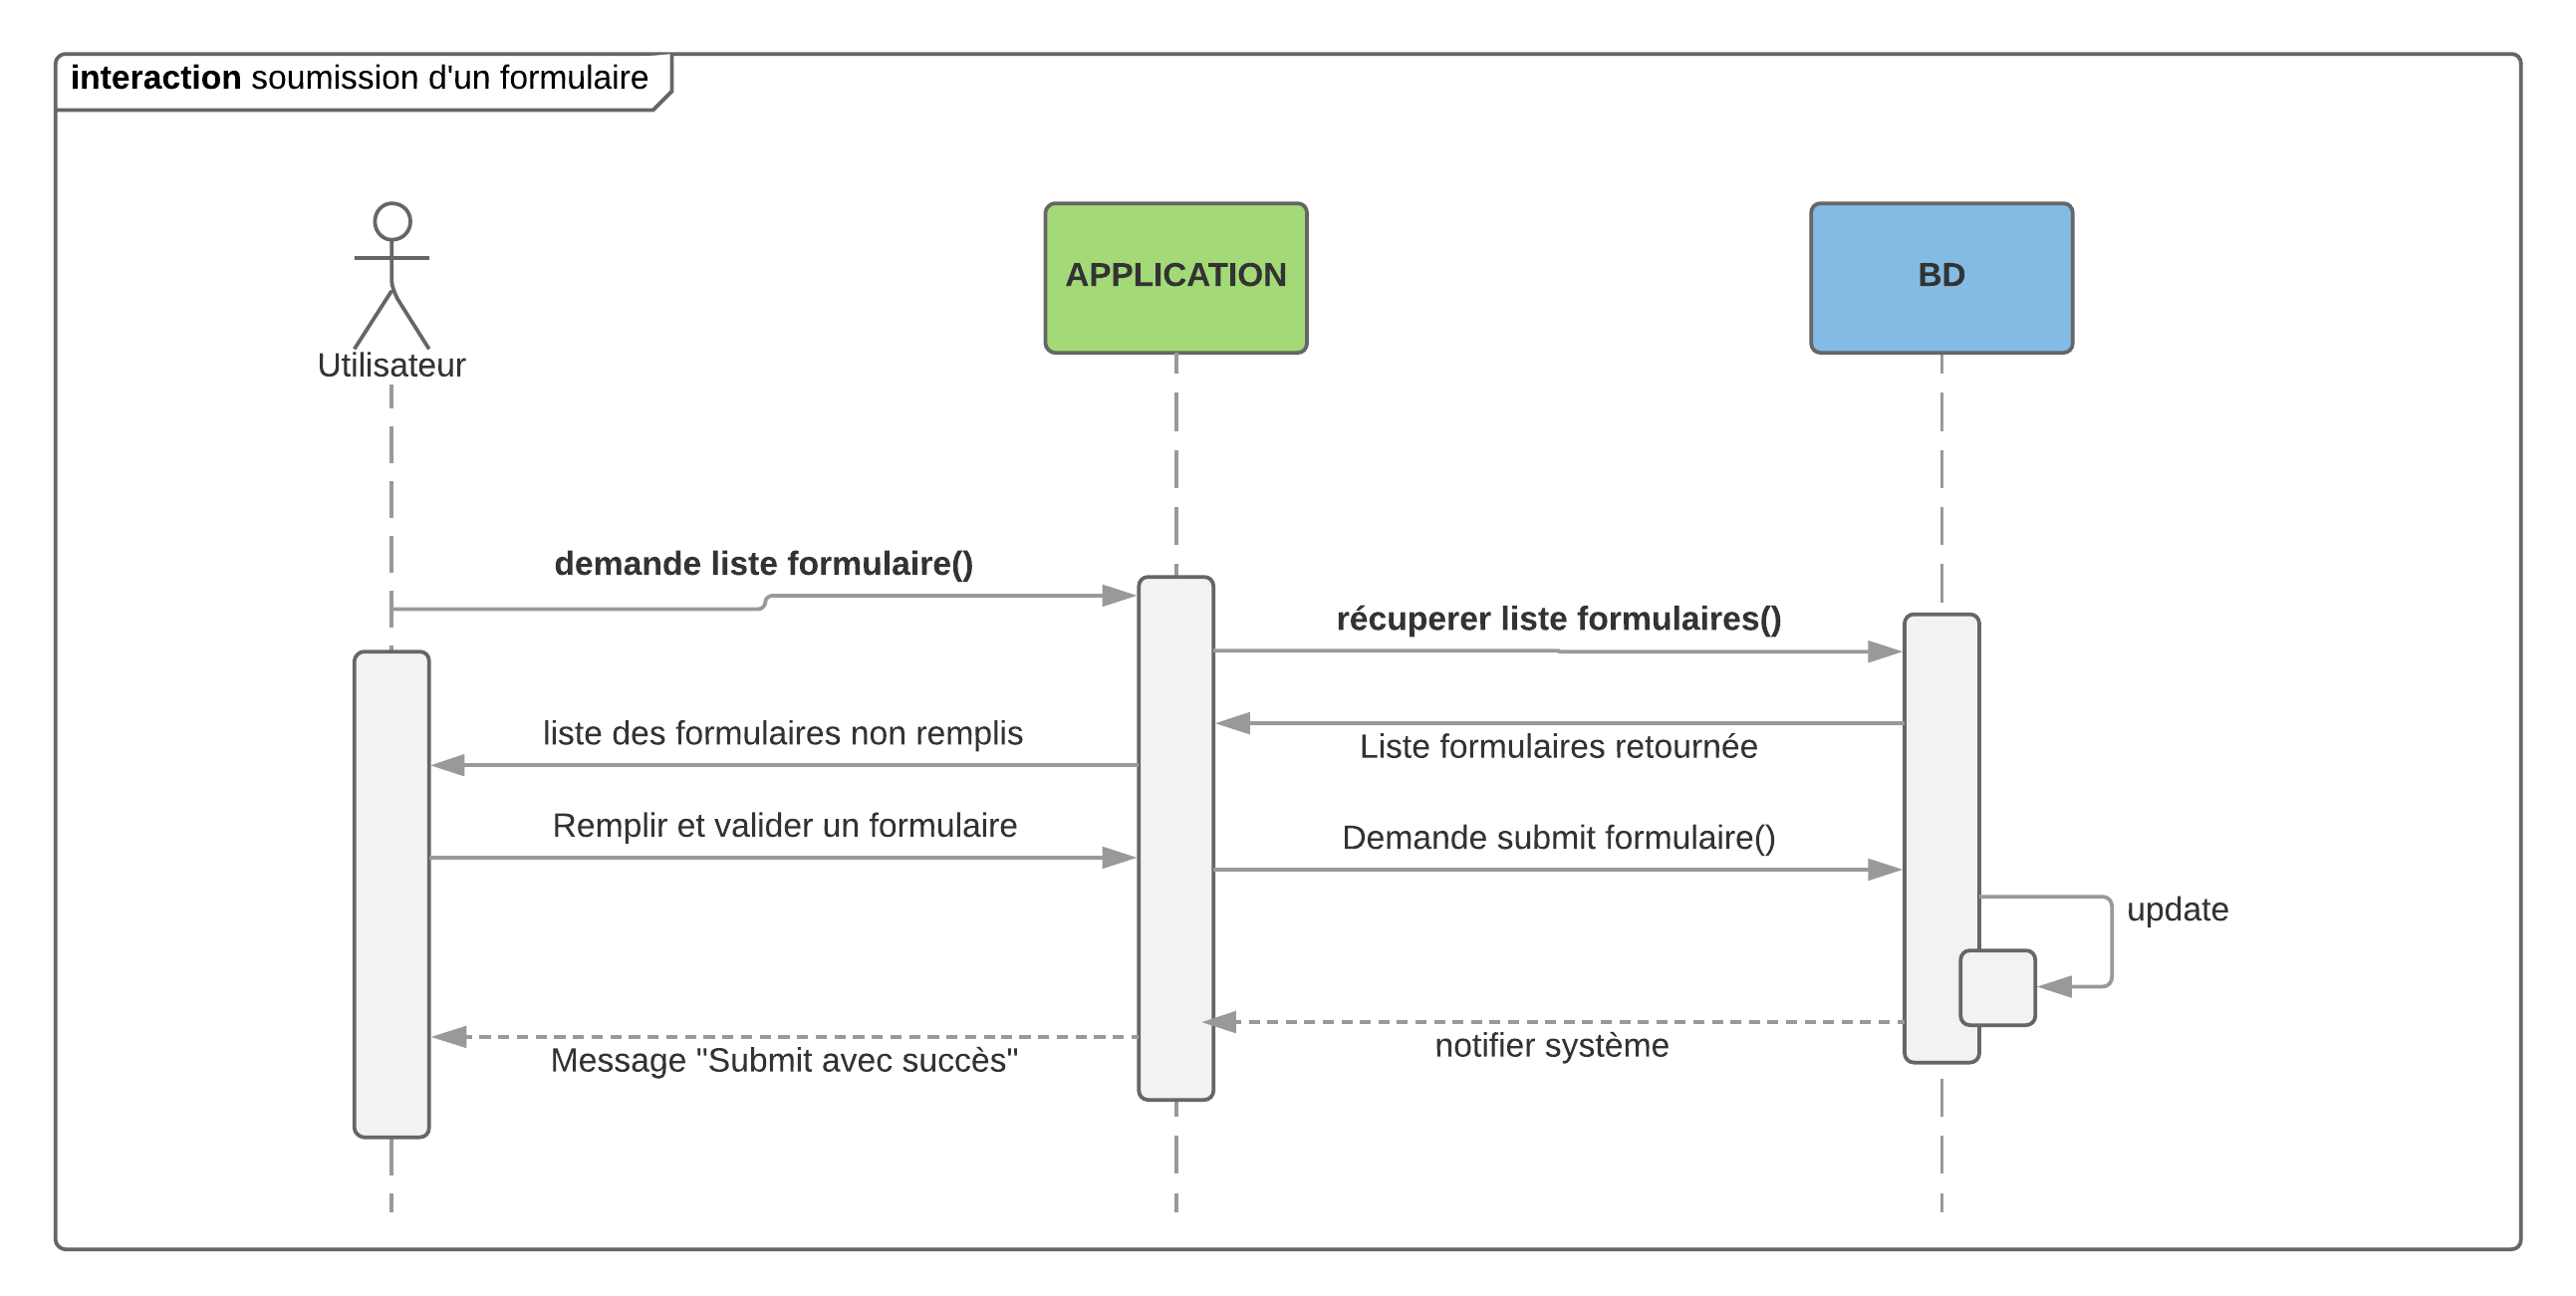
\includegraphics [width=16cm,height=7cm] {SprintImage/Diagramme_seq_formSubmit.png}
            \caption{Soumission de la réponse par le User }
            \label{fig4}
        \end{center}
    \end{figure}
\newpage
\subsection{Diagrammes de séquence système « Création formulaire »}
La figure \ref{form2} représente l’enchaînement du cas d’utilisation « Création Formulaire ».
\begin{figure} [H]
    \centering
         \begin{center}
             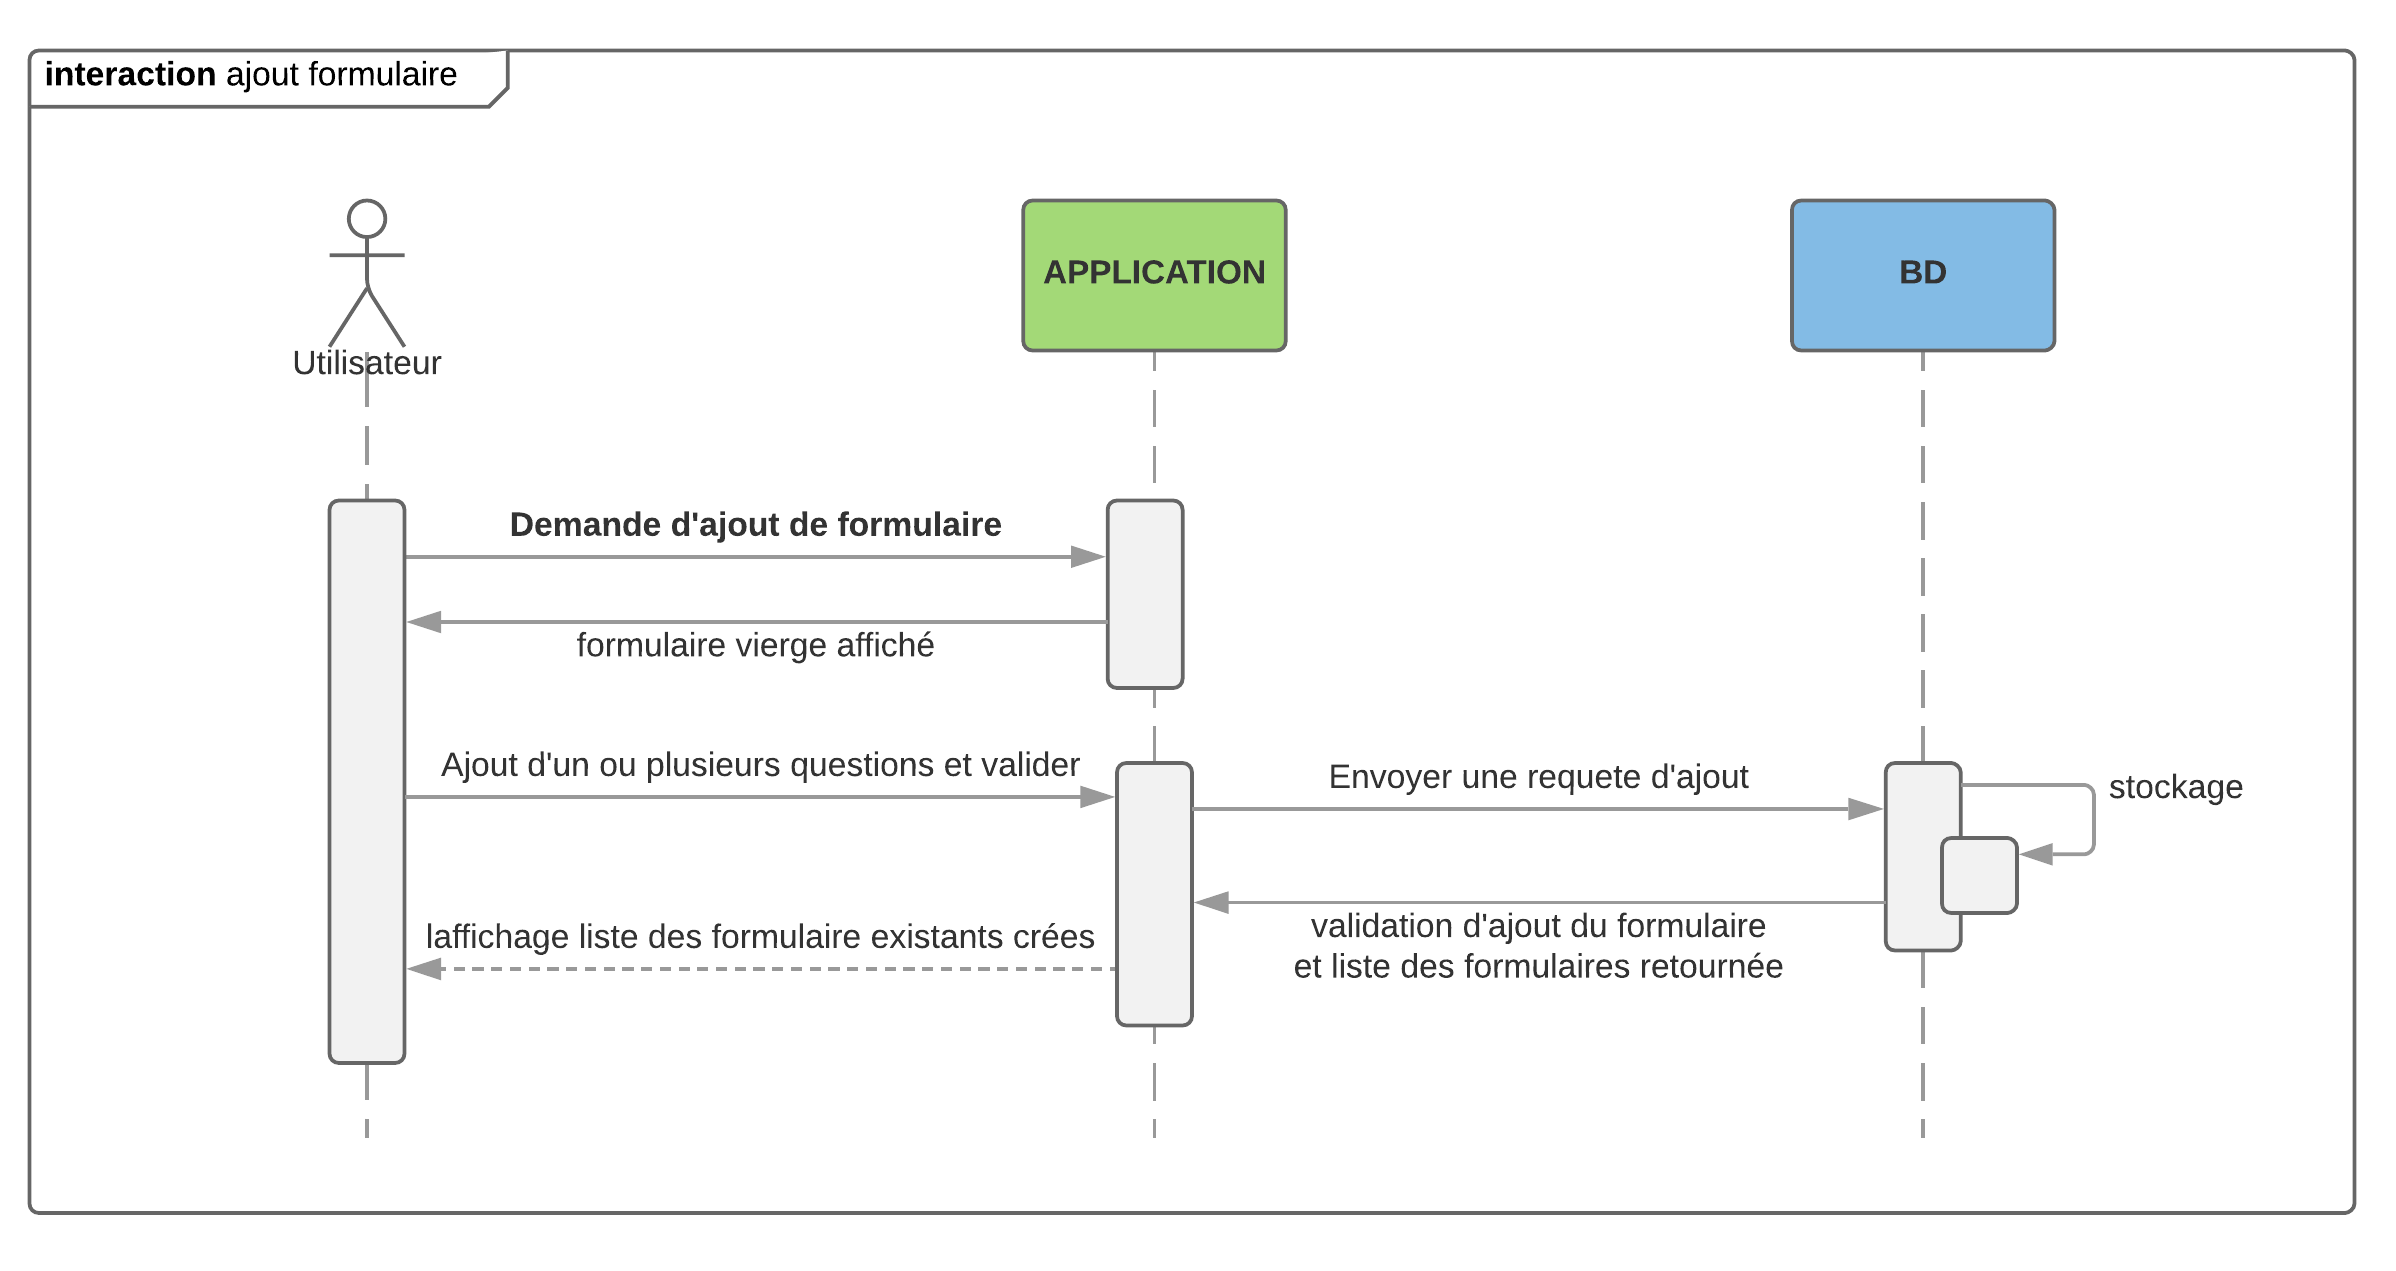
\includegraphics [width=16cm,height=9cm] {SprintImage/Diagramme_seq_ajoutForm.png}
            \caption{Mur de la création d'un formulaire}
            \label{form2}
        \end{center}
    \end{figure}
\section{Conclusion}
    Dans ce chapitre, nous avons précisé les besoins fonctionnels et non fonctionnels de l’application pour bien comprendre les différentes caractéristiques de notre système, ainsi que leur conception.
\newline
Dans le prochain chapitre, nous allons passé à la partie de réalisation des différents sprints tout en détaillant le choix des technologies utilisées.